\documentclass[11pt,a4paper]{article}

\usepackage{hyperref}
\usepackage{geometry}
\usepackage{graphicx}
\geometry{a4paper, margin=1in}

\title{State Channel Framework for On-Chain Data Betting}
\author{Paweł Nowak | Visoft}
\date{\today}

\begin{document}

\maketitle

\section*{Problem Description}

Layer 2 (L2) solutions on Ethereum face significant scalability challenges due to the shared state management by L2 sequencers for multiple applications. This shared state complicates scalability and negatively impacts performance. Additionally, the frequent requirement for cryptographic signatures from a user's wallet for each transaction slows down transactions and degrades user experience, particularly in mobile environments where seamless interaction is crucial.

\section*{Proposed Solution}

This document presents an optimized approach to state channels with a novel protocol design aimed at enhancing scalability and user interaction for blockchain applications. The core of this approach involves Central Counterparty (CC) state channels augmented by storage proofs, allowing transactions to be settled within the channel without immediate on-chain postings. This method reduces costs and increases operational efficiency.

\section*{Components Overview}

\subsection*{Server}

The server handles quote requests and ensures message integrity through secure signing. It interacts with the smart contract to validate settlements, processing transactions within the state channel efficiently and securely.

\subsection*{Client}

The client interface allows users to interact with the state channel, including initiating new channels, monitoring existing channels, and managing settlements. It provides an intuitive interface for users to manage their contracts and settlements within the state channel.

\subsection*{Cairo Smart Contract}

The Cairo Smart Contract is responsible for fund locking and event emission, ensuring secure and transparent operations within the state channel. It verifies client-server interactions via the Herodotus Integrity Verifier, maintaining transaction accuracy and integrity.

\subsection*{Proving Service}

The proving service offloads the computational task of generating proofs from the client, enhancing operational efficiency and user experience. This component is essential for the scalability and responsiveness of the system, ensuring smooth operation of the state channel framework under heavy transaction loads.

\section*{Milestones}

\subsection*{1st Milestone: Proof of Concept and Efficiency Demonstration}

\textit{Objective:} To demonstrate the architecture's ability to efficiently settle a large number of transactions using a mocked storage proof for initial settlement processes.

\begin{enumerate}
    \item \textbf{Settlement Contract:} Develop and test to ensure it can handle bulk settlements efficiently, including a mocked storage proof for demonstration purposes.
    \item \textbf{Client and Server:} Implement basic functions for initiating and managing state channels and transactions.
    \item \textbf{Proving Service:} Ensure it can generate proofs for bulk transactions, starting with mocked storage proofs to simulate the final operation.
    \item \textbf{Simulation Script:} Develop a script to simulate client behavior and generate a large volume of transactions to test settlement efficiency.
\end{enumerate}

\subsection*{Completion and Results}

The first milestone has been fully completed, successfully demonstrating the framework's ability to efficiently settle a large number of transactions. The comparison between a naive implementation and the state channel framework, as illustrated in the graph below, highlights the significant efficiency gains achieved.

\begin{figure}[h!]
    \centering
    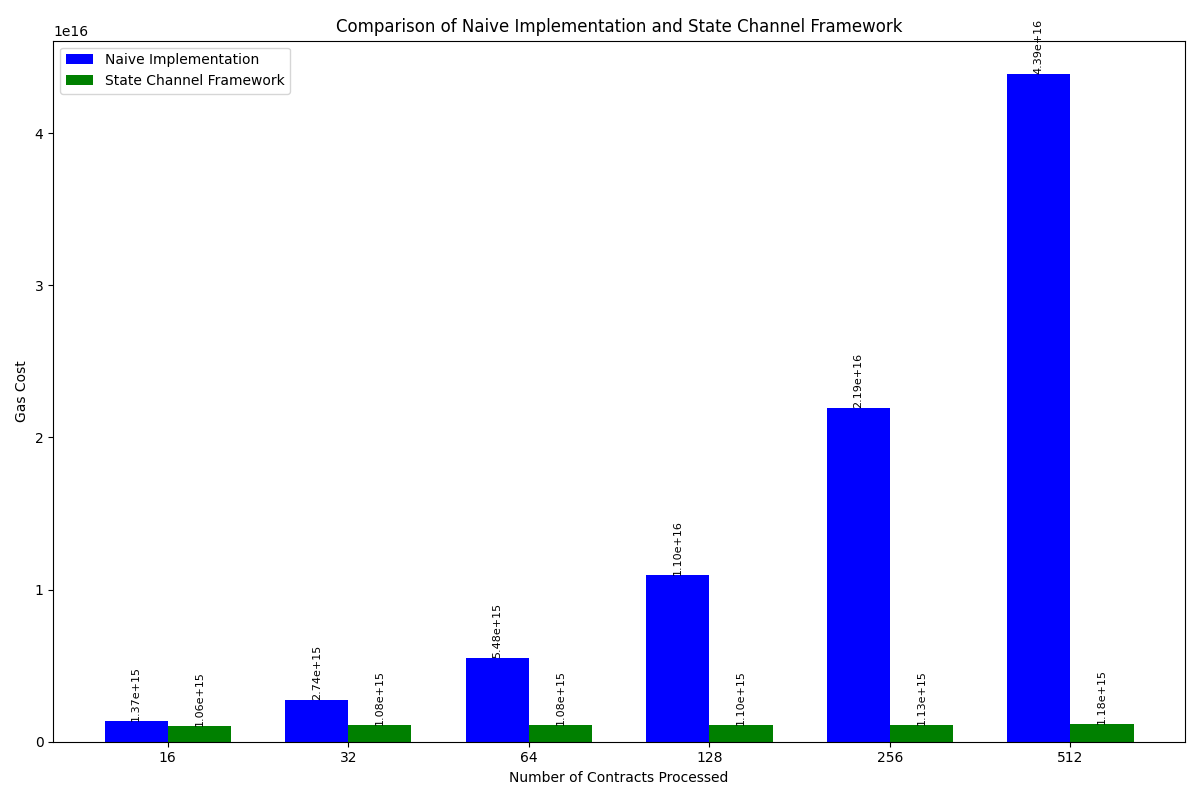
\includegraphics[width=\textwidth]{images/state-channel-framework-bench.png}
    \caption{Comparison of Naive Implementation and State Channel Framework}
    \label{fig:comparison}
\end{figure}

The graph clearly shows the gas cost savings achieved by the state channel framework compared to a naive implementation. For instance:

\begin{itemize}
    \item At 16 contracts processed, the naive implementation incurs a gas cost of approximately $1.37 \times 10^{15}$, whereas the state channel framework only uses about $1.06 \times 10^{15}$.
    \item At 128 contracts processed, the naive implementation's gas cost jumps to $1.10 \times 10^{16}$, while the state channel framework remains much lower at $1.10 \times 10^{15}$.
    \item At 512 contracts processed, the naive implementation reaches a gas cost of $4.39 \times 10^{16}$, compared to just $1.18 \times 10^{15}$ for the state channel framework.
\end{itemize}

These results demonstrate a substantial reduction in gas costs as the number of contracts processed increases, underscoring the scalability and efficiency of the state channel framework. The success of this milestone paves the way for further development and optimization, bringing us closer to a highly scalable and user-centric blockchain application.

For more details, you can visit the following repositories:
\begin{itemize}
    \item \href{https://github.com/neotheprogramist/state-channel-framework}{State Channel Framework Repository}
    \item \href{https://github.com/neotheprogramist/http-prover}{Proving Service Repository}
    \item \href{https://github.com/cartridge-gg/stone-prover/tree/docker/both-cairo-versions}{Prover Repository}
\end{itemize}

\end{document}
